\title{Dokumentacja projektu}
\author{
	Krzysztof Mizgała 262839
	\and 
	Maciej Kosierb 262239
	\and
	Wiktoria Kudła 262254
	\and
	Wiktoria Gałdusińska 262209
}
\date{\today}

\documentclass[12pt]{article}
\usepackage{hyperref}
\usepackage{polski}
\usepackage[utf8]{inputenc}
\usepackage{pgf-umlcd}

\begin{document}
	\maketitle
	
	\section{Opis projektu}\label{sec:opis-projektu}
	Nasza aplikacja służy do analizy danych finansowych.
	Korzysta z danych z https://site.financialmodelingprep.com/developer/docs/.
	Klucz API jest wymagany do uruchomienia aplikacji.
	Można go pobrać \href{https://site.financialmodelingprep.com/login}{tutaj} a następnie
	trzeba ustawić zmienną środowiskową API\_KEY do klucza.
	Można także korzystać z własnego klucza API tworząc plik .env w katalogu głównym projektu i
	dodając zmienną API\_KEY z kluczem jako wartość.

	Aplikacja pozwala na odczyt danych finansowych danej firmy.
	Używając różnych metod do zanalizowania, pokazuje wyniki i przewiduje ceny rynkowe.

	\section{Użyte technologie}\label{sec:uzyte-echnologie}
	 https://site.financialmodelingprep.com/developer/docs/ - API, z którego korzystamy.

	 Wykorzystane biblioteki Pythona:
	\begin{itemize}
		\item pandas
		\item requests
		\item dotenv
		\item PyQt5
	\end{itemize}

	Lista plików:
	\begin{itemize}
		\item analysis.py
		\item api.py
		\item docs.tex
		\item README.md
		\item requirements.txt
		\item ui.py
	\end{itemize}

	\section{Opis metod}\label{sec:uzyte-metody}
	\begin{itemize}
	\item \textit{ui.py}
		\begin{itemize}
			\item \_get\_symbols - pobiera symbole i nazwy analizowanych obiektów z pliku CSV
			\item \_init\_it - tworzy graficzny interfejs użytkownika
			\item udpate\_symbols - aktualizuje listę skrótów, kiedy kategoria jest zmieniona
			\item update\_signal - aktualizuje etykietę sygnału i kolor pudełka (?:)), kiedy sygnał jest zmieniony
			\item update\_indicators - aktualizuje listę wskaźników, kiedy pola wyboru są zmienione
			\item update\_bins - aktualizuje liczbę słupków histogramu
			\item analyze - analizuje dane dla wybranego obiektu.
			Pokazuje wyniki w postaci tabeli i wykresu świecowego
			\item \_analyze - zaczyna analizę w osobnym wątku po to, by zapobiec zacinaniu się interfejsowi
			\item draw\_plot - tworzy wykres świecowy
			\item plot\_candles - tworzy świece wykresu na osiach na podstawie dostarczonych danych
			\item plot\_indicators - tworzy wykres wskaźników, które zostały wybrane przez użytkownika, na wykresie świecowym
			\item plot\_sma - tworzy wykres wskaźników SMA na wykresie świecowym
			\item plot\_ema - tworzy wykres wskaźników EMA na wykresie świecowym
			\item plot\_bollinger - tworzy wykres wstęg Bollingera na wykresie świecowym
			\item plot\_rsi - tworzy wykres wskaźników RSI na wykresie świecowym
			\item plot\_macd - tworzy wykres wskaźników na wykresie świecowym
			\item plot\_stochastic - tworzy wykres oscylatora stochastycznego na wykresie świecowym
			\item plot\_williams - tworzy wykres \%R Williamsa
		\end{itemize}
	\end{itemize}

	\section{Diagram UML}
	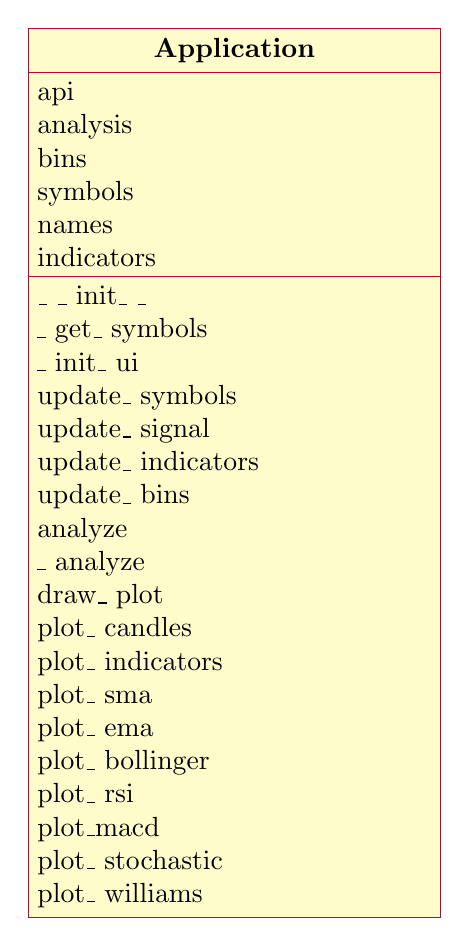
\begin{tikzpicture}
		\begin{class}{Application}{0,0}
			\attribute{api}
			\attribute{analysis}
			\attribute{bins}
			\attribute{symbols}
			\attribute{names}
			\attribute{indicators}
			\operation{\_ \_ init\_ \_}
			\operation{\_ get\_ symbols}
			\operation{\_ init\_ ui}
			\operation{update\_ symbols}
			\operation{update\_ signal}
			\operation{update\_ indicators}
			\operation{update\_ bins}
			\operation{analyze}
			\operation{\_ analyze}
			\operation{draw\_ plot}
			\operation{plot\_ candles}
			\operation{plot\_ indicators}
			\operation{plot\_ sma}
			\operation{plot\_ ema}
			\operation{plot\_ bollinger}
			\operation{plot\_ rsi}
			\operation{plot\_macd}
			\operation{plot\_ stochastic}
			\operation{plot\_ williams}
		\end{class}
	\end{tikzpicture}

\end{document}
